\begin{enumerate}[label=\thesubsection.\arabic*,ref=\thesubsection.\theenumi]
\item Find the equations of the two lines through the origin which intersect the line $ \dfrac{x-3}{2}=\dfrac{y-3}{1}=\dfrac{z}{1}$ at angles of  $\dfrac{\pi}{3}$each.
	\item
 Two lines passing through the point (2,3) intersect each other at an angle of $60\degree$. If slope of one line is 2, find the equation of the other line.
\label{chapters/11/10/3/12}
 \\
 \solution
		Using the scalar product
\begin{align}
  \cos{60\degree}=
\frac{1}{2}=\frac{\myvec{
        1&2
    }\myvec{
        1\\m
    }}{\sqrt{5}\sqrt{m^2+1}}\\
\implies 11m^2+16m-1=0\\
   or, m=\frac{-8\pm5\sqrt{3}}{11}    
\end{align}
So, the desired equation of the line is
\begin{align}
\myvec{
    \frac{-8\pm5\sqrt{3}}{11}&-1
}\vec{x} 
	&=
\myvec{
    \frac{-8\pm5\sqrt{3}}{11}&-1
}
\myvec{
    2\\3}
    \\
	&=\frac{-49\pm16\sqrt{3}}{11}
\end{align}
See 
    \figref{fig:11.10.3.12}.
\begin{figure}[!ht]
    \centering
    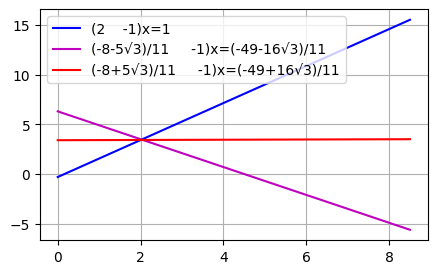
\includegraphics[width=\columnwidth]{chapters/11/10/3/12/fig/asgnt1.png}
    \caption{}
    \label{fig:11.10.3.12}
\end{figure}


\item Find the equation of the lines through the point (3, 2) which make an angle of $45\degree$  with the line $x – 2y = 3$.
\label{chapters/11/10/4/11}\\
\solution
Following the approach in \probref{chapters/11/10/3/12},
\begin{align}
\cos45\degree =
\frac{1}{\sqrt{2}} = \frac{\myvec{2 & 1} \myvec{1\\m}}{\norm{\myvec{2\\1}}\norm{\myvec{1\\m}}}
\\
\implies 
 3m^2 - 8m -3 = 0
 \\
\text{or, }
m= - \frac{1}{3}, 3
\end{align} 
Thus, the desired equations are 
\begin{align}
	\myvec{1&3}\cbrak{\vec{x}-\myvec{3\\2}}&=0\\
 \implies 	\myvec{1 & 3}\vec{x} &= 9
\end{align}
and 
\begin{align}
	\myvec{3&-1}\cbrak{\vec{x}-\myvec{3\\2}}&=0\\
		\implies 	\myvec{3 & -1}\vec{x} &= 7
\end{align}
See
\figref{fig:chapters/11/10/4/11/figs/strline.jpg}.
\begin{figure}[H]
\centering
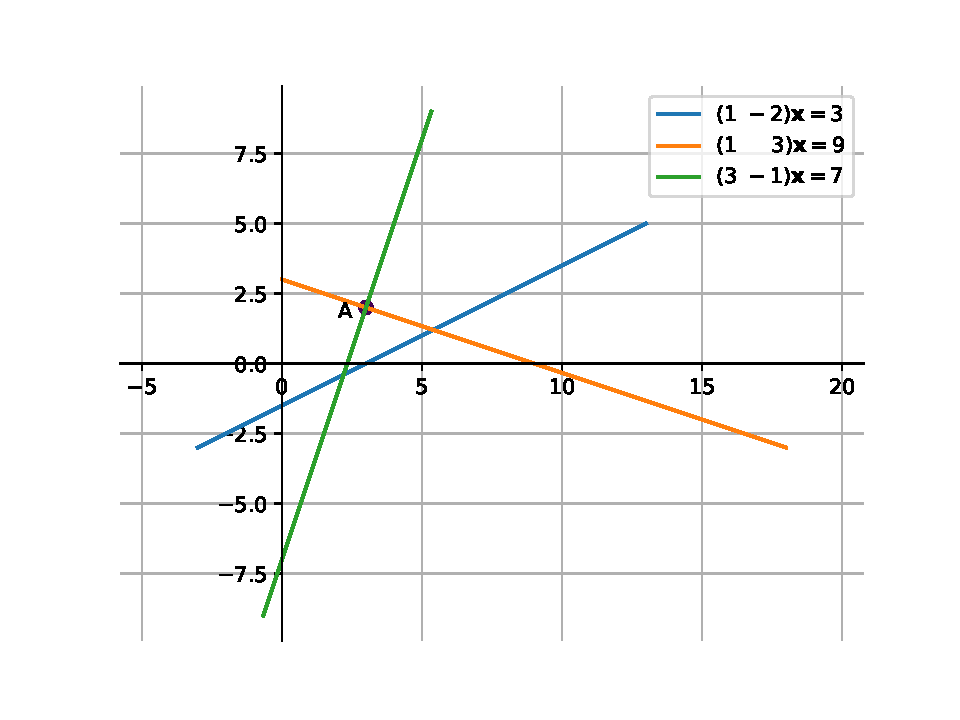
\includegraphics[width=0.75\columnwidth]{chapters/11/10/4/11/figs/fig.pdf}
\caption{}
\label{fig:chapters/11/10/4/11/figs/strline.jpg}
\end{figure}

\end{enumerate}
